%% The first command in your LaTeX source must be the \documentclass command.
%%
%% Options:
%% twocolumn : Two column layout. Do not use twocolumn for papers submitted to CEUR-WS!
%% hf: enable header and footer.
\documentclass[
% twocolumn,
% hf,
]{ceurart}


\sloppy


\usepackage{listings}
%% auto break lines
\lstset{breaklines=true}
\usepackage{subcaption}

%%
%% end of the preamble, start of the body of the document source.
\begin{document}

%%
%% Rights management information.
%% CC-BY is default license.
\copyrightyear{2026}
\copyrightclause{Copyright for this paper by its authors.
  Use permitted under Creative Commons License Attribution 4.0
  International (CC BY 4.0).}

%%
%% This command is for the conference information
\conference{Woodstock'22: Symposium on the irreproducible science,
  June 07--11, 2022, Woodstock, NY}


\title{Edge Camera based on a Single-Board Computer: Hybrid Selective Parallelization in Real-Time Video Processing}


\author[1,2]{Oleksii V. Bahatskyi}[%
orcid=0000-0003-2969-6630,
email=o.bahatskyi@kubg.edu.ua,
url=https://fitm.kubg.edu.ua/struktura1/kafedry/kafedra-kompiuternykh-nauk/sklad/936-1.html,
]
\cormark[1]

\author[1]{Kyrylo S. Malakhov}[
orcid=0000-0003-3223-9844,
email=MalakhovKS@nas.gov.ua,
url=https://linktr.ee/malakhovks,
]

\address[1]{Glushkov Institute of Cybernetics of the National Academy of Sciences of Ukraine, 40 Glushkov ave., Kyiv, 03187, Ukraine}
\address[2]{Borys Grinchenko Kyiv Metropolitan University, 18/2 Bulvarno-Kudriavska Str, Kyiv, Ukraine, 04053, Kyiv, Ukraine}

%% Footnotes
\cortext[1]{Corresponding author.}

\begin{abstract}
  This paper presents the design, implementation, and experimental evaluation of a low-cost edge camera based on a single-board computer (SBC) capable of real-time video preprocessing. The objective of the study is to assess whether a resource-constrained SBC platform can sustain real-time performance under a sequence of primitive image-processing transformations, and to determine the effectiveness of selective parallelization in achieving this goal.  A generalized hardware model of an SBC-based edge node is proposed, integrating a USB video sensor, system-on-chip processing unit, local storage, and network interface. On the software level, a user-space processing architecture implemented in C++14 and OpenCV is developed. The architecture combines a staged transformation chain with a thread pool mechanism to enable parallel execution of computationally intensive operations across multiple CPU cores. The prototype was implemented on an Orange Pi Zero 2W (Allwinner H618, quad-core Cortex-A53, 4 GB RAM) using a 640×480 USB camera stream. Three transformations—Laplacian filtering, histogram computation, and Gaussian blurring—were evaluated. Experimental results demonstrate that a fully sequential implementation achieves 24 FPS, which does not satisfy the 25 FPS real-time constraint. By parallelizing the Laplacian stage within a hybrid parallel–sequential pipeline, the system reaches 28 FPS, corresponding to a 16.7\% throughput improvement. The findings confirm that low-cost SBC platforms can function as edge nodes for lightweight real-time preprocessing tasks, provided that computational workloads are carefully structured and selectively parallelized.
\end{abstract}

\begin{keywords}
  IoT \sep
  SBC-Based Edge Camera \sep
  Single-board Computer \sep
  Real-Time Video Processing \sep
  Orange Pi Zero \sep
  Laplacian filter \sep
  Gaussian blur \sep
  OpenCV
\end{keywords}


\maketitle

\section{Introduction}

Edge computing has emerged as a fundamental architectural paradigm for distributed cyber-physical and IoT systems, particularly in scenarios involving high-volume sensor data such as video streams. In contrast to centralized cloud-based processing, edge architectures relocate computation closer to the data source, thereby reducing latency, minimizing bandwidth consumption, and improving responsiveness. For video-based systems—including surveillance, industrial monitoring, and intelligent transportation—these properties are critical for real-time analytics and event-driven decision-making.

Recent advances in \textit{single-board computers} (SBCs) have enabled the deployment of compact, low-cost devices with multi-core processors and integrated network interfaces. Such platforms provide a practical foundation for implementing edge video nodes. However, their limited computational resources impose strict constraints on achievable throughput, especially when performing continuous image transformations at standard frame rates. The central challenge is therefore to design a software architecture that maximizes performance within the boundaries of constrained hardware.

This paper examines the capacity of a low-cost SBC platform to support real-time edge-camera operation and evaluates whether selective parallelization of primitive image-processing operations is sufficient to satisfy real-time constraints. In this work, real-time operation is defined as processing each frame within the temporal budget determined by the camera frame rate. For a 25 FPS stream, this corresponds to a maximum processing time of 40 ms/frame.

The contributions of this study are threefold. First, a generalized hardware model of an SBC-based edge camera is formulated, identifying its essential architectural components. Second, a user-space processing architecture implemented in C++ and OpenCV is proposed, combining a staged transformation chain with a thread pool mechanism for intra-stage parallelism. Third, an experimental evaluation on an \textit{Orange Pi Zero 2W} platform demonstrates that hybrid parallelization increases throughput from 24 FPS to 28 FPS for the tested workload, thereby achieving real-time performance under the specified conditions.

\section{Related Works}

SBCs, particularly Raspberry Pi-class platforms and their analogues, are widely used as low-cost hardware for edge-oriented video processing and embedded computer vision. Prior studies have shown that such devices can support localized image acquisition, preprocessing, and application-specific analytics, thereby reducing dependence on centralized infrastructure and improving responsiveness in distributed video systems. In this context, SBC-based devices are increasingly treated not merely as peripheral capture units, but as compact edge nodes capable of performing nontrivial computation directly at the point of data generation.

Early work in this area demonstrated that SBC platforms can sustain basic image-processing operations for real-time applications. For example, \cite{Hiremath_Baannadabavi_Kabbin_Shirakol_2016} considered edge-detection procedures implemented on Raspberry Pi hardware, showing that compact embedded platforms can execute lightweight vision algorithms with acceptable performance characteristics. In a different application domain, Yildirim et al. \cite{Yildirim_Karaduman_Kurum_2022} investigated real-time image and video processing for in-vehicle driver assistance systems, where timely analysis of road conditions, surrounding objects, and driver behavior is required. Their study further confirmed that SBC-class devices can be used in latency-sensitive scenarios, although computational resources remain a limiting factor.

A substantial portion of the literature is devoted to intelligent surveillance and recognition tasks. Asri et al. \cite{Asri_et_al_2023} proposed an SBC-based smart security camera combining OpenCV with Haar cascade object detection and LBPH-based recognition. Similarly, Ijaradar and Xu \cite{Ijaradar_Xu_2022} developed a cost-efficient facial-recognition surveillance system for homes and small offices, in which faces are first localized in the frame and then matched against a predefined database. In a related direction, \cite{Gaddam2016FACERB} presented an attendance management system based on Raspberry Pi and OpenCV, where facial recognition was used to automate identity registration. Collectively, these studies demonstrate the practical applicability of SBC platforms to real-time surveillance, monitoring, and recognition-oriented tasks.

SBC-based image processing has also been explored in domain-specific settings beyond surveillance. In particular, \cite{Mustaffa_Khairul_2017} addressed the classification of fruits by color and size in an agricultural context, illustrating that low-cost embedded vision platforms can support specialized classification workflows. Such results confirm that SBC-based systems are sufficiently flexible to serve as computational endpoints in a broad spectrum of applied vision scenarios, provided that the processing pipeline is appropriately matched to the available hardware resources.

Beyond camera-centered studies, recent work also supports the relevance of hybrid and heterogeneous processing strategies for edge-oriented systems. Scalable ECG clustering \cite{Kaverinskiy_Chaikovsky_Mnevets_Ryzhenko_Bocharov_Malakhov_2025}, ontology- and NLP-driven intelligent systems \cite{Litvin_Velychko_Kaverinskiy_2020, Litvin_Velychko_Kaverinskiy_2022, Litvin_Palagin_Kaverinskiy_Malakhov_2023}, semantic and RDF/XML processing frameworks \cite{Palagin_Petrenko_Kaverinskiy_Malakhov_2025, Palagin_Petrenko_Malakhov_2024}, and computational modeling based on finite element analysis and process simulation \cite{Kaverinskiy_Bagliuk_Sukhenko_Verbylo_2025, Bagliuk_Kaverinskiy_2026} collectively show that modern intelligent systems increasingly depend on decomposing workloads across heterogeneous computational resources. Although these studies are not specific to SBC-based video cameras, they support the architectural premise of the present work: lightweight, latency-critical preprocessing should be executed locally on the SBC, while more computationally intensive tasks may be delegated to more capable distributed nodes.

Despite the breadth of prior work, the existing literature is predominantly oriented toward end-application functionality, such as detection, recognition, classification, or semantic processing, rather than toward the programming-level organization of the user-space processing pipeline itself. In particular, comparatively less attention has been paid to the extent to which selective parallelization of primitive transformations can shift a low-cost SBC-based vision system from near-real-time to real-time operation under an explicitly defined frame-rate constraint. The present study addresses this gap by focusing not on a specialized recognition task, but on the implementation efficiency of a lightweight C++/OpenCV processing architecture for primitive video transformations on an SBC-based edge camera.

\section{Materials and Methods}

\subsection{Real-Time Processing Criterion}
\label{subsec:subsec_3_1}

For video-processing systems, real-time operation is defined relative to the frame acquisition rate of the camera. Let $f_{\mathrm{cam}}$ denote the camera frame rate, expressed in frames per second (FPS). Then the maximum admissible processing time per frame is determined by the frame period:

\begin{equation}
	T_{\mathrm{frame}}=\frac{1}{f_{\mathrm{cam}}}.
\end{equation}

A processing system satisfies the real-time requirement if the average time required to process one frame, denoted $T_{\mathrm{proc}}$, does not exceed the available frame period:

\begin{equation}
	T_{\mathrm{proc}} \leq T_{\mathrm{frame}}=\frac{1}{f_{\mathrm{cam}}}.
\end{equation}

Equivalently, if the effective processing throughput is denoted by $f_{\mathrm{proc}}$, then the real-time condition can be written as:

\begin{equation}
	f_{\mathrm{proc}} \geq f_{\mathrm{cam}}.
\end{equation}

In the present study, the input video stream is configured at 25 FPS, which corresponds to a commonly used frame rate in video transmission standards \cite{itu_bt1197_1_1998}. Therefore, the maximum admissible processing time per frame is:

\begin{equation}
	T_{\mathrm{frame}}=\frac{1}{25}=0.04\ \mathrm{s}=40\ \mathrm{ms}.
\end{equation}

Accordingly, any implementation for which $T_{\mathrm{proc}}>40$ ms/frame is considered non-real-time under the adopted experimental conditions.

\subsection{Hardware Architecture of the SBC-Based Edge Camera}

The generalized model of the proposed edge-based camera is shown in (Figure~\ref{fig:figure_1}). The model is derived from the earlier concept of an intelligent video camera \cite{Bahatskyi_2018} and is adapted here to the requirements of edge-oriented deployment. The architecture consists of four principal components.

\begin{figure}[htbp] % use [t] or [htbp] if you prefer normal floating
	\centering
	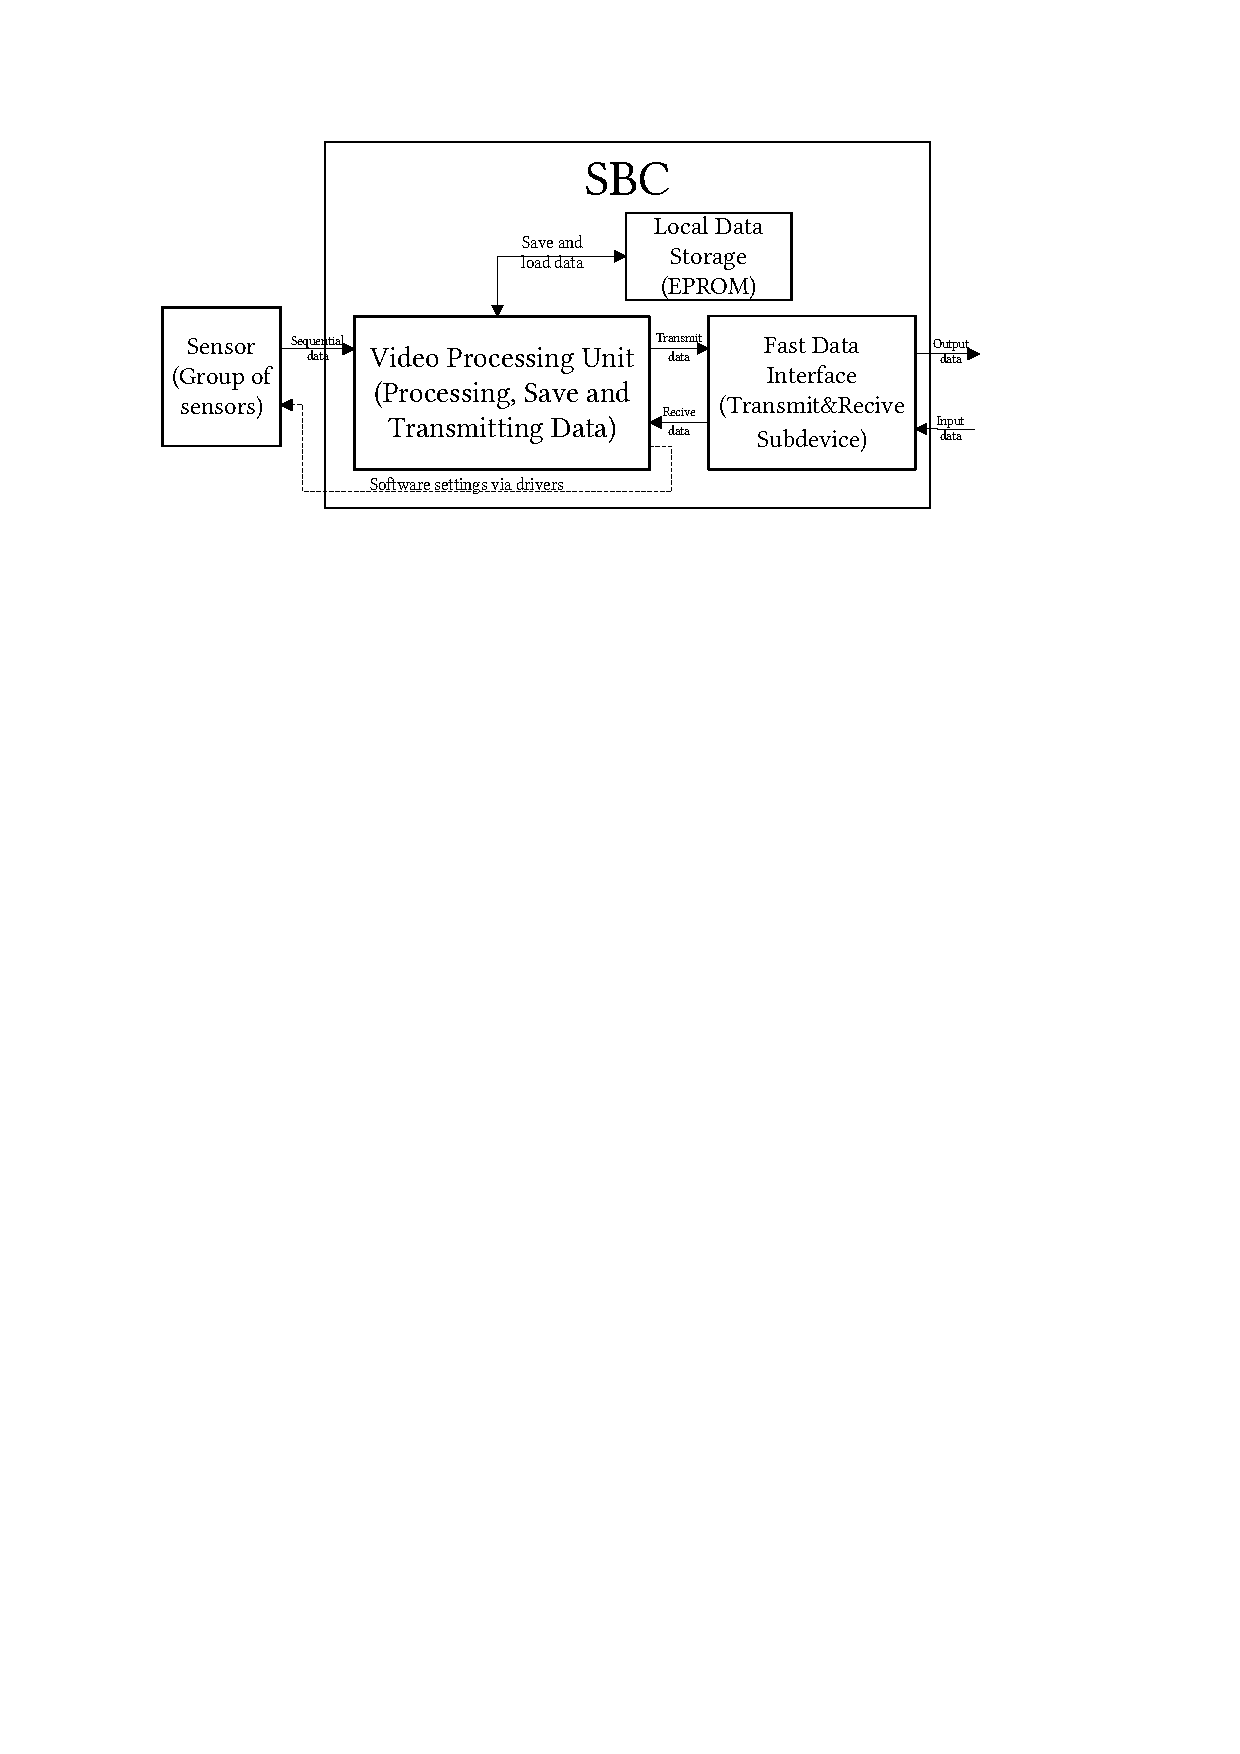
\includegraphics[width=0.8\linewidth,keepaspectratio]{figure_1.pdf}
	\caption{The generalized model of the proposed edge-based camera.}
	\label{fig:figure_1}
\end{figure}

The first component is the \textit{sensor subsystem}, which acquires the video stream and delivers it to the processing node. Depending on the implementation, the sensor may be connected via dedicated interfaces such as CSI or via general-purpose interfaces such as USB. The sensor may also be represented by a single camera or by a group of coordinated sensing devices \cite{Popovic_Seyid_Cogal_Akin_Leblebici_2017}.

The second component is the \textit{video processing unit}, which performs frame acquisition, transformation, and intermediate analysis. In the SBC-based implementation considered in this work, this role is performed by a system-on-chip (SoC) integrating multiple CPU cores and auxiliary processing resources.

The third component is the \textit{local storage subsystem}, which provides persistent or temporary storage for the operating system, application binaries, intermediate results, and diagnostic data. In low-cost SBC configurations, this functionality is typically implemented using microSD or eMMC storage.

The fourth component is the \textbf{communication interface}, which transmits the processing results or selected frame data to external systems. In the simplest implementation, this function is provided by the integrated Ethernet or Wi-Fi interface of the SBC, although more advanced communication subsystems are also possible \cite{Zhang_Tao_2021}.

Thus, an SBC-based edge camera integrates sensing, local computation, storage, and communication within a compact and low-cost platform. However, the practical effectiveness of such a node depends critically on the software stack and on the computational organization of the video-processing workflow

\subsection{Software Stack and Device Interface}

The basic software layer of the proposed system is a Linux-based operating system, which provides hardware abstraction, driver support, process scheduling, and memory management for user-space applications. In SBC platforms of the considered class, Linux distributions such as Ubuntu are commonly used due to their hardware support and compatibility with standard vision libraries.

Communication with the camera device is organized through the standardized Video4Linux2 (V4L2) interface \cite{schimek2024v4l2}, which provides system-level access to video capture devices and enables frame acquisition from the user-space application. This interface serves as the boundary between the camera hardware and the application-level processing logic implemented in C++.

The user-space application was developed in ISO/IEC 14882:2014-compliant C++ using the OpenCV library. This combination was selected because it provides low-level control over execution flow, support for efficient memory handling, compatibility with multithreaded programming, and a mature implementation base for image-processing operations.

\subsection{User-Space Processing Architecture}

The proposed user-space processing architecture is organized as a staged frame-processing workflow implemented in C++ and OpenCV, as shown in (Figure~\ref{fig:figure_2}). Each input frame passes through a fixed sequence of transformations, and the result of each stage is forwarded to the next stage until the full processing chain is completed.

The architecture combines a transformation chain based on the Chain of Responsibility pattern \cite{qi2010chain} with a ThreadPool mechanism for bounded parallel execution \cite{Puyda_2025}. The transformation chain defines the processing order, whereas the thread pool enables selected stages to exploit multiple CPU cores.

In the hybrid implementation, only computationally intensive transformations are parallelized. For such stages, the input frame is partitioned into fragments processed concurrently by worker threads, after which the partial results are merged. The remaining stages are executed sequentially. This design, schematically presented in (Figure~\ref{fig:figure_2}), reduces processing time without introducing unnecessary synchronization overhead and is therefore well suited to resource-constrained SBC platforms.

\begin{figure}[htbp] % use [t] or [htbp] if you prefer normal floating
	\centering
	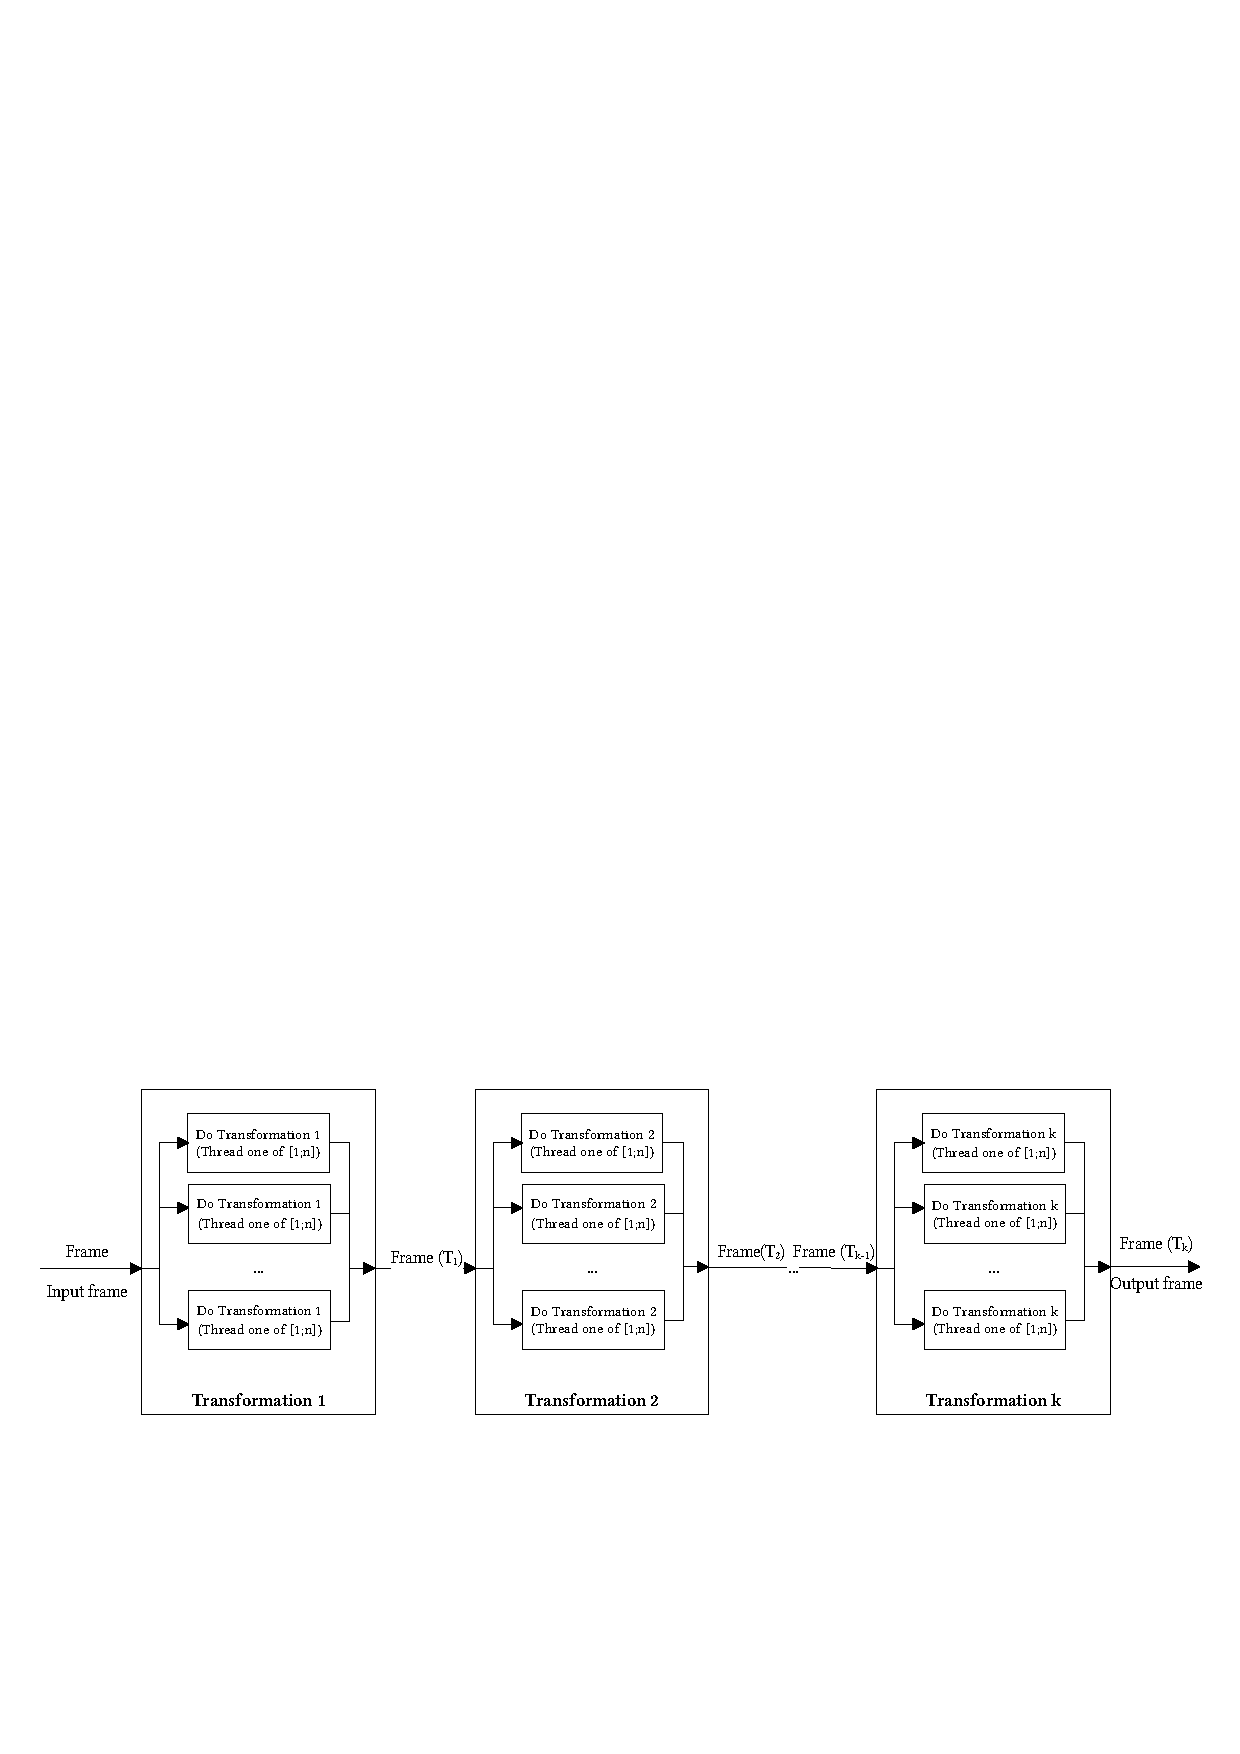
\includegraphics[width=\linewidth,keepaspectratio]{figure_2.pdf}
	\caption{The proposed user-space processing architecture.}
	\label{fig:figure_2}
\end{figure}

\subsection{Primitive Video Transformations}

Since the target hardware is a low-cost SBC, the methodological focus of this study is limited to primitive image transformations that are representative, computationally meaningful, and implementable under constrained resources.

The first transformation is \textit{Gaussian blurring}, which performs local smoothing by convolving the image with a Gaussian kernel. This operation reduces high-frequency noise and is frequently used as a preprocessing step in vision pipelines \cite{reinhard2006hdr}.

The second transformation is \textit{Laplacian-based contour extraction} \cite{Viola_Jones_2001}. The Laplacian operator is a second-order differential operator that emphasizes regions of rapid intensity variation and is therefore suitable for highlighting edges and structural transitions in the image. In the present study, a discrete $3 \\times 3$ approximation of the Laplacian operator is used. The result is stored as a grayscale frame for subsequent analysis.

The third transformation is \textit{histogram computation}, which determines the distribution of pixel intensities in the frame. Histograms are widely used as compact descriptors of image structure and may support subsequent tasks such as object localization, motion characterization, or scene-change analysis \cite{Lowe_2004}.

These operations were selected because they represent common low-level vision procedures while remaining sufficiently lightweight for controlled evaluation on SBC hardware.

\subsection{Experimental Platform and Implementation Details}

The experimental prototype was implemented using an \textit{Orange Pi Zero 2W} SBC equipped with an \textit{Allwinner H618} processor (quad-core ARM Cortex-A53 at 1.5 GHz) and 4 GB RAM \cite{orangepi_zero2w_manual}. The operating system was \textit{Ubuntu 22.04.4 LTS} with Linux kernel 6.1.31-sun50iw9. Persistent storage was provided by a 64 GB Class 10 microSD card.

Video acquisition was performed using a \textit{Logitech C170 USB camera} configured for a frame resolution of 640 × 480 pixels with YUYV color encoding \cite{logitech_c170_guide}. The application was compiled directly on the SBC using g++ 12.3.0 with support for the C++14 standard \cite{isoiec14882_2014}. The computer-vision functionality was implemented using \textit{OpenCV 4.10}.

The experimental application was developed to evaluate the compliance of the hardware-software configuration with the real-time criterion defined in Subsection~\ref{subsec:subsec_3_1}. The implemented transformation chain consisted of three stages: Gaussian blurring, Laplacian filtering, histogram computation.

%\begin{equation}
%	\phi_1 = \text{Laplacian filtering},
%	\qquad
%	\phi_2 = \text{histogram computation},
%	\qquad
%	\phi_3 = \text{Gaussian blurring}.
%\end{equation}

The Laplacian stage employed the OpenCV \textit{filter2D} function with the $3 \times 3$ mask:

\begin{equation}
	\mathbf{K}_{\mathrm{Lap}}=
	\begin{bmatrix}
		0 & -1 & 0 \\
		-1 & 4 & -1 \\
		0 & -1 & 0
	\end{bmatrix}.
\end{equation}

Histogram computation was implemented using \textit{calcHist}, and Gaussian smoothing was implemented using \textit{GaussianBlur} with a $3 \times 3$ kernel. The application allows the number of execution threads to be specified for transformations that admit partitioned processing. The measured output metric is the average achieved FPS, displayed during execution and used as the primary performance indicator.

Two execution modes were considered. In the first mode, all three transformations were executed sequentially, yielding a baseline implementation. In the second mode, the Laplacian stage was parallelized across CPU cores, while the remaining two stages were executed sequentially. This hybrid configuration was selected to assess whether selective parallelization of the most computationally intensive stage is sufficient to satisfy the real-time criterion on the target platform.

\section{Results}

Two execution modes were evaluated. In the first mode, all three transformations were executed sequentially. In the second mode, a hybrid parallel-sequential configuration was applied, in which the Laplacian filtering stage was parallelized across the available CPU cores of the SBC, whereas histogram computation and Gaussian blurring remained sequential. This design made it possible to assess whether selective parallelization of the most computationally intensive transformation is sufficient to achieve real-time performance on the target platform.

In the fully sequential configuration, the developed application achieved an average throughput of 24 FPS, as illustrated in (Figure~\ref{fig:figure_3}). This value corresponds to an average processing time of approximately 41.7 ms per frame, which exceeds the admissible threshold of 40 ms per frame for a 25 FPS stream. Therefore, the purely sequential implementation does not satisfy the adopted real-time requirement.

In the hybrid parallel-sequential configuration, the application achieved an average throughput of 28 FPS, as shown in (Figure~\ref{fig:figure_4}). This corresponds to an average processing time of approximately 35.7 ms/frame, which is below the admissible 40 ms limit. Under the experimental conditions of this study, the hybrid configuration therefore satisfies the real-time criterion.

The reported results were obtained using the proposed software architecture based on the \textit{Chain of Responsibility} and \textit{ThreadPool} patterns. However, not all primitive transformation stages benefit from parallelization; for some stages, thread-management overhead may outweigh the performance gain.

\begin{figure}[htbp]
	\centering
	\begin{subfigure}{0.4\linewidth}
		\centering
		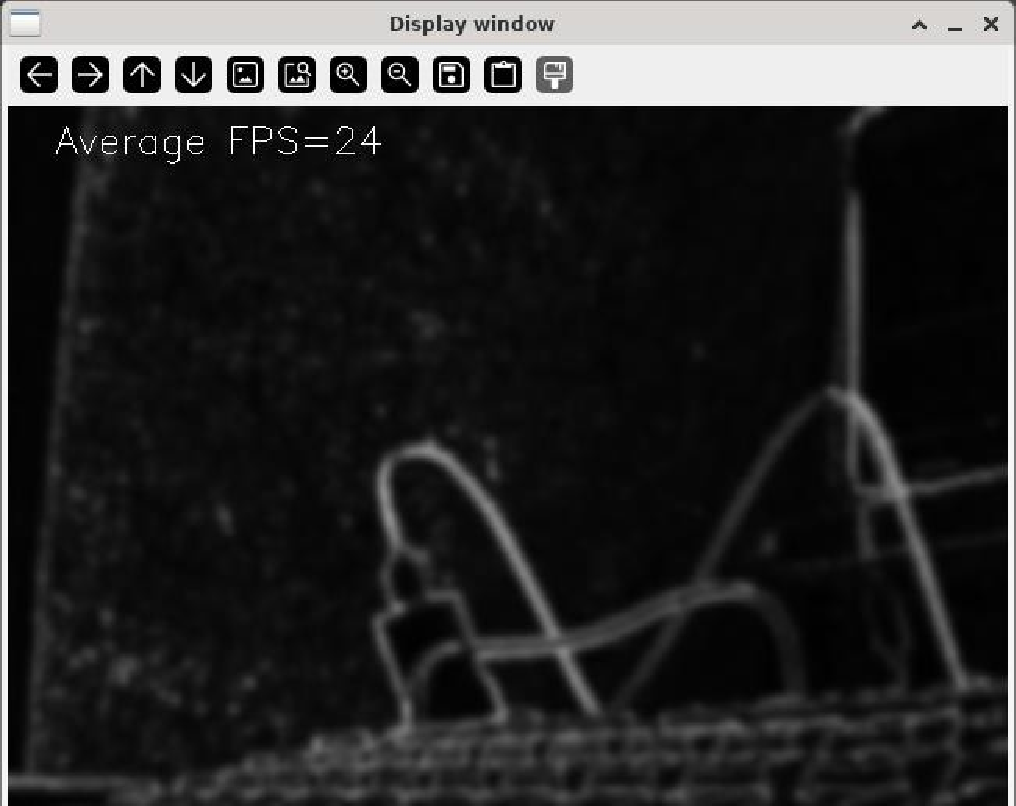
\includegraphics[width=\linewidth,keepaspectratio]{figure_3.pdf}
		\caption{Full sequential primitive transformation.}
		\label{fig:figure_3}
	\end{subfigure}\hfill
	\begin{subfigure}{0.4\linewidth}
		\centering
		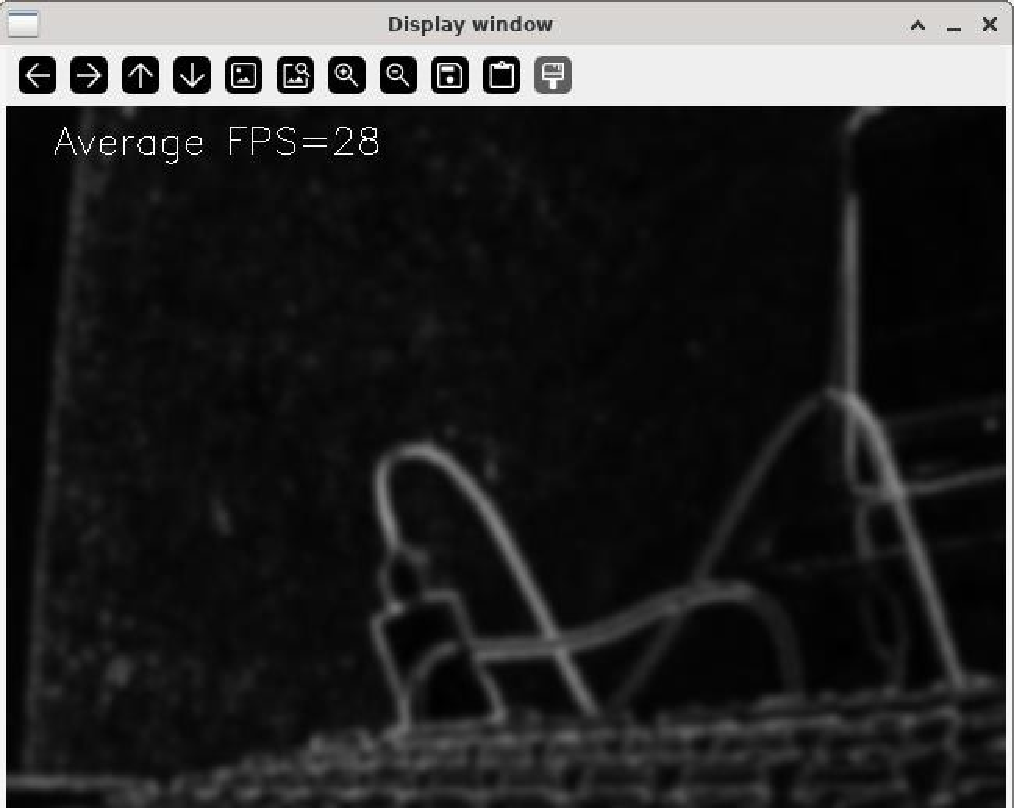
\includegraphics[width=\linewidth,keepaspectratio]{figure_4.pdf}
		\caption{Hybrid primitive transformation.}
		\label{fig:figure_4}
	\end{subfigure}
	\caption{Comparison of sequential and hybrid frame-processing modes.}
	\label{fig:comparison_modes}
\end{figure}

A comparison of the two execution modes shows that selective parallelization of the Laplacian stage increased throughput from 24 FPS to 28 FPS. This corresponds to a relative improvement of approximately 16.7\%. The obtained result indicates that even partial parallelization of a single transformation stage can produce a measurable gain in end-to-end processing performance on a low-cost SBC platform.

The results also show that the proposed architecture is suitable for lightweight edge-side preprocessing tasks, particularly those based on primitive image transformations. At the same time, the observed performance margin remains limited, which suggests that more computationally demanding operations would likely require either additional optimization, lower-resolution input, hardware acceleration, or partial offloading to more powerful nodes within a distributed edge architecture. Thus, the experimental findings support the use of low-cost SBC-based cameras as compact edge nodes for simple real-time preprocessing tasks, while also indicating the practical limits of such devices under constrained computational resources.

\begin{table}[ht]
	\centering
	\caption{Performance comparison of the evaluated processing modes}
	\label{tab:performance_comparison}
	\begin{tabular}{lccc}
		\hline
		\textbf{Execution mode} & \textbf{Average FPS} & \textbf{Processing time per frame (ms)} & \textbf{Real-time criterion} \\
		\hline
		Sequential & 24 & 41.7 & Not satisfied \\
		Hybrid     & 28 & 35.7 & Satisfied \\
		\hline
	\end{tabular}
\end{table}


\section{Discussion}

The obtained results are consistent with the edge-computing paradigm, since the proposed system performs latency-sensitive preprocessing directly on the SBC near the data source, without requiring continuous transmission of raw video to external infrastructure. This organization reduces communication overhead and demonstrates that even a low-cost edge node can satisfy a real-time requirement for lightweight video transformations when the workload is structured appropriately and selectively parallelized.

At the same time, the present study has several limitations. The evaluation was conducted on a single SBC platform, with one USB camera configuration, one input resolution ($640 \times 480$), and a limited set of three primitive image transformations. The experiments focused on average throughput (FPS) and did not examine energy consumption, thermal effects, long-duration stability, network transmission performance, or more computationally demanding computer-vision tasks.

\section{Conclusion}

This paper investigated a low-cost SBC-based edge camera for real-time video preprocessing. The experimental results showed that the sequential implementation achieved 24 FPS, whereas the proposed hybrid parallel-sequential approach increased performance to 28 FPS, thereby satisfying the adopted real-time criterion for a 25 FPS stream.

These findings indicate that low-cost SBC platforms are suitable for lightweight edge-side video preprocessing, although more computationally demanding tasks would require additional optimization or more capable hardware.

\section{CRediT Author Statement}

OB: Conceptualization, Methodology, Software, Data curation, Writing -- Original draft preparation. KM: Validation, Visualization, Writing -- Reviewing and Editing.

\section*{Funding}

These results were obtained as part of the project “Develop a hardware-software system for video data processing in different frequency ranges using edge computing” (State registration No.~0126U000623; \url{https://dir.ukrintei.ua/view/rk/3afdf57cf0459c15c1ca946d8e2a1a5a}), funded by the NAS of Ukraine.

Additional support was provided by the R\&D projects ``To develop theoretical foundations and a functional model of a computer for processing complex information structures'' (State registration No.~0124U002317; \url{https://nrat.ukrintei.ua/searchdoc/0124U002317/}) and ``Develop Means of Supporting Virtualization Technologies and Their Use in Computer Engineering and Other Applications'' (State registration No.~0124U001826; \url{https://nrat.ukrintei.ua/en/searchdoc/0124U001826}), funded by the NAS of Ukraine.

\section{Data Availability Statement}

The data and source code supporting the findings of this study are available from the authors upon reasonable request.

\section*{Declaration on Generative AI}

During the preparation of this work, the authors used \textit{gpt-oss-120b} (OpenAI’s open-weights LLM), deployed locally on institutional hardware, solely for grammar and spelling checks.

\bibliography{ceur_ref}


\end{document}